\documentclass[a4paper,12pt]{article}
\usepackage[slovene]{babel}
\usepackage[utf8]{inputenc}
\usepackage[T1]{fontenc}
\usepackage{lmodern}
\usepackage{amsmath}
\usepackage{amsthm}
\usepackage{url}
\usepackage{graphicx}
\usepackage{booktabs} % za lepše tabele
\usepackage{multirow} % za vnose v tabeli čez več vrstic

% Nastavimo koliko prostora izpustimo pod napisom nad sliko ali tabelo.
\setlength{\belowcaptionskip}{2mm}
% Nastavimo odmik prve vrstice v odstavku na 0mm.
\setlength{\parindent}{0mm}
% Definicija okolij izrek, posledica
{\theoremstyle{plain}
\newtheorem{izrek}{Izrek}
}


% Definicija okoli za definicije in vaje
{\theoremstyle{definition}
\newtheorem {definicija}{Definicija}
}
\newcommand{\pojem}[1]{\emph{\color{purple}#1}}
%%%%%%%%%%%%%%%%%%%%%%%%%%%%%%%%%%%%%%%%%%%%%%%%%%%%%%%%%%%%%%%%%%%%%%%%
% Prvi sklop nalog
%%%%%%%%%%%%%%%%%%%%%%%%%%%%%%%%%%%%%%%%%%%%%%%%%%%%%%%%%%%%%%%%%%%%%%%%

\title{Magični kvadrati}
\author{}
\date{}
% 1. naloga
% Glavo dokumenta popravite tako, da se ne bo izpisal datum.
% To naredite tako, da za ukazom `\title` dodate ukaz `\date{}`.

\begin{document}
\maketitle
\begin{center}
   \includegraphics{slika.pdf}
\end{center}

  

% 2. naloga
% Na tem mestu vključite sliko `slika.pdf`:
% - naredite okolje `center`, da bo slika postavljena na sredino
% - v okolju `center' uporabite ukaz  `\includegraphics{slika.pdf}`

Prirejeno iz virov:

% 3. naloga
% Za izpis spletnih naslovov morate uporabiti ukaz `\url`.
% S tem ukazom lahko izpišete en spletni naslov tako,
% naslov podate kot argument ukaza `\url` v zavitih oklepajih.
% V spodnjem okolju `itemize` ukaz `\url` na obeh spletnih naslovih
% (naslova sta v komentarju, da ne pride do napake pri prevajanju te datoteke).
\begin{itemize}
   \item \url{http://en.wikipedia.org/wiki/Magic_square}
   \item \url{http://mathworld.wolfram.com/MagicSquare.html}
\end{itemize}

% 4. naloga
% Na tem mestu uporabite ukaz, ki izpiše kazalo vsebine.
% Poiščite ga na spletu: po angleško se kazalu vsebine reče "table of contents".
\tableofcontents
%%%%%%%%%%%%%%%%%%%%%%%%%%%%%%%%%%%%%%%%%%%%%%%%%%%%%%%%%%%%%%%%%%%%%%%%
% Konec prvega sklopa nalog
%%%%%%%%%%%%%%%%%%%%%%%%%%%%%%%%%%%%%%%%%%%%%%%%%%%%%%%%%%%%%%%%%%%%%%%%

% Z ukazom `\newpage` lahko povzročite prehod na novo stran.
\newpage

\section{Uvod}

\begin{definicija}
   \emph{Magični kvadrat} reda $n$ je nabor $n^2$ različnih števil,
   ki so razvrščena v kvadratno tabelo tako, da vedno dobimo enako vsoto,
   če seštejemo vsa števila poljubne vrstice, vsa števila poljubnega
   stolpca ali vsa števila v katerikoli od glavnih diagonal.
\end{definicija}

Primer magičnega kvadrata reda 3 je prikazan v tabeli \ref{tab:mag3}.

% - napis nad tabelo: Magični kvadrat reda 3
% - oznaka: table:mag3
% Začetek magičnega kvadrata
\begin{table}[!ht]
   \caption{Magični kvadrat reda 3}
   \centering
   \begin{tabular}{|c|c|c|}
      \hline
      8 & 1 & 6 \\ \hline
      3 & 5 & 7 \\ \hline
      4 & 9 & 2 \\ \hline
   \end{tabular}
   \label{tab:mag3}
\end{table}

% Konec magičnega kvadrata

\begin{definicija}
   Magični kvadrat reda $n$ je \emph{normalen}, če v njem nastopajo števila
   \begin{equation}
      % oznaka: eq:numbers
      1, 2, 3, \ldots, n^2-1, n^2.
   \end{equation}
   \label{eq:numbers}
\end{definicija}

Magični kvadrat v tabeli \ref{tab:mag3} je normalen.
To je tudi najmanjši netrivialen normalen magični kvadrat.
Poleg normalnih magičnih kvadratov so zanimivi tudi magični kvadrati praštevil.

%%%%%%%%%%%%%%%%%%%%%%%%%%%%%%%%%%%%%%%%%%%%%%%%%%%%%%%%%%%%%%%%%%%%%%%%

\section{Zgodovina}

\subsection{Kvadrat ">Lo Shu"<}

Kitajska literatura iz časa vsaj 2800 let pred našim štetjem govori o legendi
\emph{Lo Shu} -- ">zvitek reke Lo"<. V antični Kitajski je prišlo do
silne poplave. Ljudje so skušali rečnemu bogu narasle reke Lo ponuditi daritev,
da bi pomirili njegovo jezo. Iz vode se je prikazala želva z zanimivim vzorcem
na oklepu: v tabeli velikosti tri krat tri so bila predstavljena števila, tako
da je bila vsota števil v katerikoli vrstici, kateremkoli stolpcu in na obeh
glavnih diagonalah enaka: 15. To število je tudi enako številu dni v 24 ciklih
kitajskega sončnega leta. Ta vzorec so na določen način uporabljali upravljalci
reke.

% - napis nad tabelo: Kvadrat Lo Shu
% - oznaka: table:loshu
% Začetek magičnega kvadrata
\begin{table}[!ht]
   \caption{Kvadrat Lo Shu}
   \centering
   \begin{tabular}{|c|c|c|}
      \hline
         4 & 9 & 2 \\\hline
         3 & 5 & 7 \\\hline
         8 & 1 & 6 \\\hline
      \end{tabular}
      \label{tab:loshu}
\end{table}
% Konec magičnega kvadrata

%%%%%%%%%%%%%%%%%%%%%%%%%%%%%%%%%%%%%%%%%%%%%%%%%%%%%%%%%%%%%%%%%%%%%%%%

\subsection{Kulturna pomembnost}

Magični kvadrati so fascinirali človeštvo skozi vso zgodovino. Najdemo jih
v številnih kulturah, npr.\ v Egiptu in Indiji, vklesane v kamen ali
kovino, uporabljane kot talismane za dolgo življensko dobo in v
izogib boleznim.

\emph{Kubera-Kolam} je talna poslikava, ki se uporablja v Indiji, in je v
obliki magičnega kvadrata reda 3. Ta je v bistvu enak kot kvadrat
Lo Shu, vendar je vsako število povečano za 19.

% - napis nad tabelo: Kvadrat Kubera-Kolam
% - oznaka: table:kubera
% Konec magičnega kvadrata
\begin{table}[!ht]
   \caption{Kvadrat Kubera-Kolam}
   \centering
   \begin{tabular}{|c|c|c|}
      \hline
         23 & 28 & 21 \\\hline
         22 & 24 & 26 \\\hline
         27 & 20 & 25 \\\hline
       
      \end{tabular}
      \label{tab:kubera}
\end{table}
% Konec magičnega kvadrata

Z magičnimi kvadrati so se ukvarjali tudi najbolj znani matematiki kot na
primer Euler, glej \cite{euler}. % ključ: euler

%%%%%%%%%%%%%%%%%%%%%%%%%%%%%%%%%%%%%%%%%%%%%%%%%%%%%%%%%%%%%%%%%%%%%%%%

\subsection{Zgodnji kvadrati reda 4}

Najzgodnejši znani magični kvadrat reda 4 je bil odkrit na napisu
v Khajurahu v Indiji in v Enciklopediji Bratovščine Čistosti iz enajstega
ali dvanajstega stoletja. Vrh vsega gre celo za ">panmagični kvadrat"<.
V Evropi sta morda najbolj znana naslednja magična kvadrata reda 4:

Magični kvadrat v litografiji Melancholia I (glej sliko \ref{fig:durer}
za izsek s kvadratom) Albrechta Dürerja naj bi bil najzgodnejši magični kvadrat
v evropski umetnosti. Zelo podoben je kvadratu Yang Huija, ki je nastal na Kitajskem
približno 250 let pred Dürerjevim časom. 
% Tu vstavite sliko
% - napis nad sliko: Dürerjev magični kvadrat
% - oznaka: fig:durer
% Dodatni parameter v oglatih oglepajih sliko nastavi velikost
% slike na 150% originalne velikosti.
\begin{figure}[!ht]
   \centering
   \caption{Dürerjev magični kvadrat}
   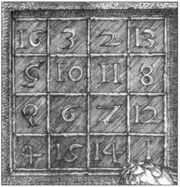
\includegraphics[scale=1.5]{durer.png}
   \label{fig:durer}
\end{figure}

Vsoto 34 je mogoče najti pri seštevanju števil v vsaki vrstici, vsakem stolpcu,
na vsaki diagonali, v vsakem od štirih kvadrantov, v sredinskih štirih poljih,
v štirih kotih, v štirih sosedih kotov v smeri urinega kazalca ($3+8+14+9$), v
štirih sosedih kotov v nasprotni smeri urinega kazalca ($2+5+15+12$), v dveh naborih
simetričnih parov ($2+8+9+15$ in $3+5+12+14$), in še na nekaj drugih načinov.
Števili na sredini spodnje vrstici tvorita letnico litografije: 1514.
%
% - napis nad tabelo: Dürerjev magični kvadrat $4\times 4$
% - oznaka: table:durer
%   16 &  3 &  2 & 13 \\\hline
%    5 & 10 & 11 &  8 \\\hline
%    9 &  6 &  7 & 12 \\\hline
%    4 & 15 & 14 &  1 \\\hline
\begin{table}[!ht]
   \caption{Dürerjev magični kvadrat $4\times 4$}
   \centering
   \begin{tabular}{|c|c|c|c|}
      \hline
   16 &  3 &  2 & 13 \\\hline
    5 & 10 & 11 &  8 \\\hline
    9 &  6 &  7 & 12 \\\hline
    4 & 15 & 14 &  1 \\\hline
      \end{tabular}
      \label{tab:durer}
\end{table}

Pasijonska fasada na katedrali Sagrada família v Barceloni
(glej sliko \ref{fig:sagrada} za fotografijo) vsebuje magični kvadrat reda 4.
% sklic: fig:sagrada

% Tu vstavite sliko
% - napis nad sliko: Pasijonska fasada, Sagrada Família
% - oznaka: fig:sagrada
\begin{figure}[!ht]
   \centering
\caption{Pasijonska fasada, Sagrada Família}
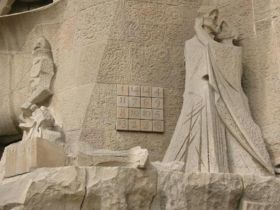
\includegraphics[scale=0.5]{sagrada.png}
   \label{fig:sagrada}
\end{figure}

Vsota števil v vrsticah, stolpcih oziroma na diagonalah je 33 -- Jezusova starost
v času pasijona. Strukturno je kvadrat podoben Dürerjevemu, vendar so števila
v štirih poljih zmanjšana za 1. Posledica je, da sta števili 10 in 14 podvojeni
in zato kvadrat ni normalen.
%
% - napis nad tabelo: Pasijonska fasada, Sagrada Família
% - oznaka: table:sagrada
%    1 & 14 & 14 &  4 \\\hline
%   11 &  7 &  6 &  9 \\\hline
%    8 & 10 & 10 &  5 \\\hline
%   13 &  2 &  3 & 15 \\\hline
\begin{table}[!ht]
   \caption{Pasijonska fasada, Sagrada Família}
   \centering
   \begin{tabular}{|c|c|c|c|}
      \hline
    1 & 14 & 14 &  4 \\\hline
  11 &  7 &  6 &  9 \\\hline
   8 & 10 & 10 &  5 \\\hline
  13 &  2 &  3 & 15 \\\hline
      \end{tabular}
      \label{tab:sagrada}
\end{table}

%%%%%%%%%%%%%%%%%%%%%%%%%%%%%%%%%%%%%%%%%%%%%%%%%%%%%%%%%%%%%%%%%%%%%%%%

\section{Osnovne lastnosti}

\begin{definicija}
      Vsoto ene vrstice, enega stolpca ali ene od glavnih diagonal
      v magičnem kvadratu imenujemo \emph{magična konstanta}.
\end{definicija}

% Začetek okolja izrek
   Magična konstanta normalnega magičnega kvadrata reda $n$
   je enaka
   \begin{equation}
      % oznaka: eq:mc
      \mathcal{M}_2(n) = \frac{1}{2} n(n^2+1)
   \end{equation}
% Konec okolja izrek

% Začetek dokaza
   V normalnem magičnem kvadratu reda $n$ je vsota vseh nastopajočih
   števil (glej \eqref{eq:numbers} na strani \ref{eq:numbers}) enaka
   $1+2+3+\dots+n^2=\sum_{k=1}^{n^2}k=\frac{1}{2}n^2(n^2+1)$. Ker imamo
   v kvadratu $n$ vrstic z enako vsoto, je vsota števil v eni vrstici
   enaka številu $\mathcal{M}_2(n)$. 
% Konec dokaza

Preprost račun pokaže, da je konstanti \eqref{eq:numbers} analogna konstanta
$\mathcal{M}_2(n;A,D)$ za magični kvadrat, v katerem so nameščena števila
$A$, $A+D$, $A+2D$, \dots, $A+(n^2-1)D$, enaka \label{eq:mc}.

Kvadratu v tabeli \ref{tab:closhu} ustrezata konstanti $A=20$ in $D=1$.

\begin{definicija}
      Če vsako od števil v normalnem magičnem kvadratu reda $n$ odštejemo
      od števila $n^2+1$, dobimo nov magični kvadrat, ki je prvotnemu
      \emph{komplementaren}.
\end{definicija}

Na primer, magičnemu kvadratu Lo Shu (glej tabelo \ref{tab:loshu}) priredimo
komplementarni kvadrat, prikazan v tabeli \ref{tab:closhu}.
%
% - napis nad tabelo: Kvadratu Lo Shu komplementarni kvadrat
% - oznaka: ttable:closhu
%   6 & 1 & 8 \\\hline
%   7 & 5 & 3 \\\hline
%   2 & 9 & 4 \\\hline
\begin{table}[!ht]
   \caption{Kvadratu Lo Shu komplementarni kvadrat}
   \centering
   \begin{tabular}{|c|c|c|}
      \hline

         6 & 1 & 8 \\\hline
         7 & 5 & 3 \\\hline
         2 & 9 & 4 \\\hline
         \end{tabular}
      \label{tab:closhu}
\end{table}

Vidimo, da je dobljeni kvadrat moč dobiti iz kvadrata Lo Shu tudi z zasukom za
180 stopinj okrog središča, kvadrat iz tabele \ref{tab:closhu} pa je mogoče dobiti
iz kvadrata Lo Shu z zrcaljenjem preko sredinske vodoravne črte.

Število različnih normalnih magičnih kvadratov

\begin{definicija}
      Pravimo, da sta dva magična kvadrata \emph{različna}, če enega ni mogoče dobiti
      iz drugega s pomočjo zasukov oziroma zrcaljenj.
\end{definicija}

Števila različnih normalnih magičnih kvadratov se nahajajo v tabeli \ref{tab:stevila}.

% - napis nad tabelo: Število različnih normalnih magičnih kvadratov
% - oznaka: table:stevila
% Začetek tabele
\begin{table}[!ht]
   \caption{Število različnih normalnih magičnih kvadratov}
   \centering
   \begin{tabular}{lcccccc}\toprule
      &\multicolumn{5}{c}{točna vrednost} &  približek\\\midrule
         red & 1 & 2 & 3 & 4 & 5 & 6  \\\midrule
         število kvadratov & 1 & 0 & 1 & 880 & 275305224 & $(1,7745\pm 0,0016)10^{19}$\\
      \bottomrule
   \end{tabular}
   \label{tab:stevila}
\end{table}
% Konec tabele

Vse normalne magične kvadrate reda 4 je oštevilčil Frénicle de Bessy
leta 1693, glej \cite{bessy}, in jih je moč najti v knjigi \cite{berlekamp}
iz leta 1982. Število normalnih kvadratov reda 5 je izračunal
R. Schroeppel leta 1973 (glej Gardner \cite{gardner}).
Natančno število vseh različnih normalnih magičnih kvadratov reda 6 ni znano.
Avtorja navedenega približka sta Pinn in Wieczerkowski (glej \cite{pinn}), ki
sta za oceno uporabila simulacijo Monte Carlo in metode statistične mehanike.
 % ključi: bessy, berlekamp, gardner, pinn

%%%%%%%%%%%%%%%%%%%%%%%%%%%%%%%%%%%%%%%%%%%%%%%%%%%%%%%%%%%%%%%%%%%%%%%%

\section{Primeri}

V tabelah \ref{tab:mag5}, \ref{tab:mag6} in \ref{tab:mag9} so prikazani
magični kvadrati redov 5, 6 in 9.
\begin{table}[!ht]
   \caption{Magični kvadrat reda 5}
\centering
\begin{tabular}{|c|c|c|c|c|}
   \hline
   17 & 24 &  1 &  8 & 15 \\\hline
   23 &  5 &  7 & 14 & 16 \\\hline
    4 &  6 & 13 & 20 & 22 \\\hline
   10 & 12 & 19 & 21 &  3 \\\hline
   11 & 18 & 25 &  2 &  9 \\\hline
\end{tabular}
\label{tab:mag5}
\end{table}
\begin{table}[!ht]
   \caption{Magični kvadrat reda 6}
\centering
\begin{tabular}{|c|c|c|c|c|c|}
   \hline
    6 & 32 &  3 & 34 & 35 &  1 \\\hline
    7 & 11 & 27 & 28 &  8 & 30 \\\hline
   19 & 14 & 16 & 15 & 23 & 24 \\\hline
   18 & 20 & 22 & 21 & 17 & 13 \\\hline
   25 & 29 & 10 &  9 & 26 & 12 \\\hline
   36 &  5 & 33 &  4 &  2 & 31 \\\hline
\end{tabular}
\label{tab:mag6}
\end{table}
\begin{table}[!ht]
   \caption{Magični kvadrat reda 9}
\centering
\begin{tabular}{|c|c|c|c|c|c|c|c|c|}
   \hline
   47 & 58 & 69 & 80 &  1 & 12 & 23 & 34 & 45 \\\hline
   57 & 68 & 79 &  9 & 11 & 22 & 33 & 44 & 46 \\\hline
   67 & 78 &  8 & 10 & 21 & 32 & 43 & 54 & 56 \\\hline
   77 &  7 & 18 & 20 & 31 & 42 & 53 & 55 & 66 \\\hline
    6 & 17 & 19 & 30 & 41 & 52 & 63 & 65 & 76 \\\hline
   16 & 27 & 29 & 40 & 51 & 62 & 64 & 75 &  5 \\\hline
   26 & 28 & 39 & 50 & 61 & 72 & 74 &  4 & 15 \\\hline
   36 & 38 & 49 & 60 & 71 & 73 &  3 & 14 & 25 \\\hline
   37 & 48 & 59 & 70 & 81 &  2 & 13 & 24 & 35 \\\hline
\end{tabular}
\label{tab:mag9}
\end{table}
% - napis nad tabelo: Magični kvadrat reda 5
% - oznaka: table:mag5
%   17 & 24 &  1 &  8 & 15 \\\hline
%   23 &  5 &  7 & 14 & 16 \\\hline
%    4 &  6 & 13 & 20 & 22 \\\hline
%   10 & 12 & 19 & 21 &  3 \\\hline
%   11 & 18 & 25 &  2 &  9 \\\hline

% - napis nad tabelo: Magični kvadrat reda 6
% - oznaka: table:mag6
%    6 & 32 &  3 & 34 & 35 &  1 \\\hline
%    7 & 11 & 27 & 28 &  8 & 30 \\\hline
%   19 & 14 & 16 & 15 & 23 & 24 \\\hline
%   18 & 20 & 22 & 21 & 17 & 13 \\\hline
%   25 & 29 & 10 &  9 & 26 & 12 \\\hline
%   36 &  5 & 33 &  4 &  2 & 31 \\\hline

% - napis nad tabelo: Magični kvadrat reda 9
% - oznaka: table:mag9
%   47 & 58 & 69 & 80 &  1 & 12 & 23 & 34 & 45 \\\hline
%   57 & 68 & 79 &  9 & 11 & 22 & 33 & 44 & 46 \\\hline
%   67 & 78 &  8 & 10 & 21 & 32 & 43 & 54 & 56 \\\hline
%   77 &  7 & 18 & 20 & 31 & 42 & 53 & 55 & 66 \\\hline
%    6 & 17 & 19 & 30 & 41 & 52 & 63 & 65 & 76 \\\hline
%   16 & 27 & 29 & 40 & 51 & 62 & 64 & 75 &  5 \\\hline
%   26 & 28 & 39 & 50 & 61 & 72 & 74 &  4 & 15 \\\hline
%   36 & 38 & 49 & 60 & 71 & 73 &  3 & 14 & 25 \\\hline
%   37 & 48 & 59 & 70 & 81 &  2 & 13 & 24 & 35 \\\hline

%%%%%%%%%%%%%%%%%%%%%%%%%%%%%%%%%%%%%%%%%%%%%%%%%%%%%%%%%%%%%%%%%%%%%%%%

\newpage
\bibliographystyle{siam}
\bibliography{magic.bib}
% Tu vstavite bibliografijo

%%%%%%%%%%%%%%%%%%%%%%%%%%%%%%%%%%%%%%%%%%%%%%%%%%%%%%%%%%%%%%%%%%%%%%%%

\end{document}
